% !TEX root = main.tex

\section{频域率滤波}
\subsection{傅里叶级数与傅里叶变换}
\begin{definition}[傅里叶级数]
$f(t)$为以$T$为周期的函数,绝对可积
\[f(t)=\sum_{n=-\infty}^{\infty}c(n)\ee^{j\frac{2\pi n}{T}t}\]
其中
\[c(n)=\frac{1}{T}\intabu{-T/2}{T/2}{f(t)\ee^{-j\frac{2\pi n}{T}t}}{t},\,n=0,\pm 1,\pm 2,\ldots\]
\end{definition}

傅里叶级数中每一个基函数都是一个单频谐波,对应的系数(频谱)表明原函数对这种频率成分贡献的大小(原函数在这个谐波上的投影)
\[a_k=\frac{1}{T}\intab{0}{T}{f(x)\cdot\ee^{-jk\frac{2\pi}{T}x}}\]

\begin{definition}[冲激]
某一点处积分为无穷
\[\delta(t)=\begin{cases}
\infty & t=0\\
0 & t\ne 0
\end{cases}\]
即
\[\intab{-\infty}{\infty}{\delta(t)}=1\]
具有取样(sifting)特性
\[\intab{-\infty}{\infty}{f(t)\delta(t)}=f(0)\]
\end{definition}
\begin{definition}[冲激串]
无限多个分离的周期冲激单元$\Delta T$之和
\[s_{\Delta T}(t)=\sum_{-\infty}^{\infty}\delta(x-n\Delta T)\]
\end{definition}
\begin{figure}[H]
\centering
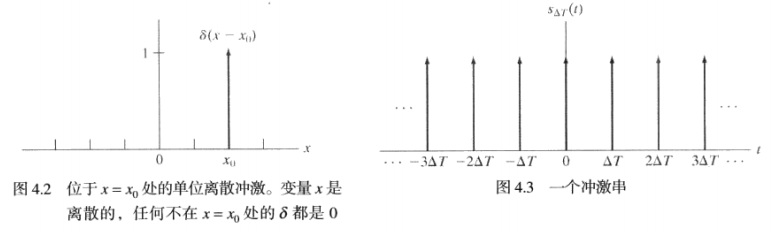
\includegraphics[width=0.8\linewidth]{fig/impulse.png}
\end{figure}

\begin{definition}[傅里叶变换与反变换]
傅里叶变换
\[F(u)=\intabu{-\infty}{+\infty}{f(t)\ee^{-j 2\pi ut}{t}}\]
反变换
\[f(t)=\intabu{-\infty}{+\infty}{F(u)\ee^{j 2\pi ut}{u}}\]
\end{definition}
由于傅里叶变换是$f(t)$乘上正弦项的展开,正弦项的频率由$\mu$决定(变量$t$已经被积分),积分后只剩下频率,故称傅里叶变换域是频率域。
\begin{example}
矩形函数
\[f(t)=\begin{cases}
A & -W/2\leq t\leq W/2\\
0 & \text{otherwise}
\end{cases}\]
的傅里叶变换为
\[F(u)=\intabu{-W/2}{W/2}{A\ee^{-j2\pi ut}}{t}=AW\frac{\sin(\pi\mu W)}{\pi\mu W}=AW\sinc(\mu W)\]
\end{example}

\begin{definition}[卷积]
\[f(t)*h(t)=\intabu{-\infty}{+\infty}{f(\tau)h(t-\tau)}{\tau}\]
\end{definition}
\begin{theorem}[卷积定理]
建立起空间域和频率域的联系
\[f(t)*h(t)\iff F(\mu)H(\mu)\]
且
\[f(t)h(t)\iff F(\mu)*H(\mu)\]
即空间域两个函数卷积的傅里叶变换等于两个函数的傅里叶变换在频率域的乘积
\end{theorem}


\subsection{取样函数}
模拟取样
\[\tilde{f}(t)=f(t)s_{\Delta T}(t)=\sum_{n=-\infty}^\infty f(t)\delta(t-n\Delta T)\]
可以得到采样函数$\tilde{f}(t)$的傅里叶变换$\tilde{F}(u)$为
\[\tilde{F}(u)=\mF\{\tilde{f}(t)\}=\mF\{f(t)s_{\Delta T}(t)\}=F(u)*S(u)\]
其中
\[S(u)=\frac{1}{\Delta T}\sum_{n=-\infty}^{\infty}\delta\lrp{u-\frac{n}{\Delta T}}\]
进而
\[\tilde{F}(u)=F(u)*S(u)=\intabu{-\infty}{\infty}{F(\tau)S(u-\tau)}{\tau}=\frac{1}{\Delta T}\sum_{n=-\infty}^{\infty}F\lrp{u-\frac{n}{\Delta T}}\]
\begin{theorem}[奈奎斯特(Nyquist)采样定理]
如果以超过函数最高频率的两倍的采样率来获得样本,则连续的带限函数可以完全从它的样本集恢复,即
\[\frac{1}{\Delta T}>2\mu_{\max}\]
\end{theorem}

若以低于两倍的采样率来采样则会出现混淆现象
\begin{figure}[H]
\centering
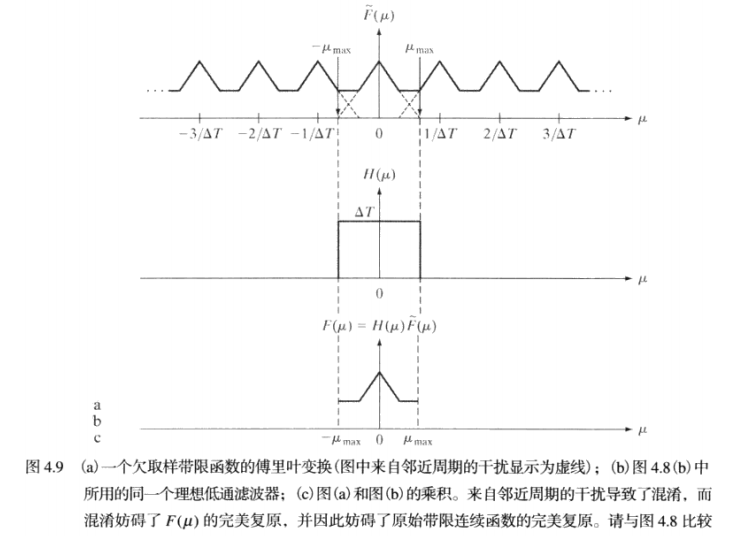
\includegraphics[width=\linewidth]{fig/nyquist.png}
\end{figure}

空间域表达式
\[f(t)=\sum_{n=-\infty}^{\infty}f(n\Delta T)\sinc[(t-n\Delta T)/\Delta T]\]

\subsection{单变量的离散傅里叶变换}
\[|F(u)|^2=F(u)\cdot F^\star(u)\]